\section{Data}
    \subsection{Data sources}
    
    The full TCGA-BRCA RNA-sequencing dataset was downloaded from the GDC data portal using R/Bioincuctor package TCGAbiolinks v2.8.13
\cite{Colaprico2016}. Table \ref{table:full} shows the overview of samples collected by the TCGA research network. 

     %   TABLE 2.1
     
            \begin{table}[!htbp]
            \centering
            \caption{RNA-Seq samples from TCGA-BRCA dataset. Full and final dataset sample count is shown}
            \label{table:full}          
            \begin{tabular}{cc|c|c|c}
            \multicolumn{1}{l}{} & \textbf{Samples} & \textbf{Tumour} & \textbf{Normal} & \textbf{Metastasis} \\ \cline{2-5} 
            \multicolumn{1}{c|}{\textbf{\begin{tabular}[c]{@{}c@{}}Full\\  dataset\end{tabular}}} & 1212 & \begin{tabular}[c]{@{}c@{}}1093\\ (F: 1081, M: 12)\end{tabular} & \begin{tabular}[c]{@{}c@{}}112\\ (F: 112, M :0)\end{tabular} & \multicolumn{1}{c|}{\begin{tabular}[c]{@{}c@{}}7\\ (F: 7, M: 0)\end{tabular}} \\ \hline
            \multicolumn{1}{c|}{\textbf{\begin{tabular}[c]{@{}c@{}}Final\\  dataset\end{tabular}}} & 969 & F:857 & F:112 & \multicolumn{1}{l|}{} \\ \cline{2-5} 
            \end{tabular}
            \end{table}
                 

    The original dataset has been subset to a more manageable collection of samples based of three main factors, which entailed including samples that \textbf{ i)} are female only (to reduce biological variation coming from gender) \textbf{ii)} are present in the list of manually curated samples and their classifications \textbf{iii)} are provided with enough metadata to benefit exploratory analysis. Only primary tumour and normal samples were included in the analysis.
    
    The curated lists of samples specifying stage and morphological type of samples were provided by the collaborators from other groups at DCRC.Table \ref{table:morphstage} shows the number of samples that were represented in the morphological groups and stages in the final dataset. 
    
    
     %   TABLE 2.2
            \begin{table}[!htbp]
            \centering
            \caption{The number of samples in each morphology type and stage in the final datset. 'Stage X' is unknown/unidentifiable stage. 'Other morphologies' comprised various other mophologies that are represented by only a few samples each}
            \label{table:morphstage}
            \begin{tabular}{lccllclc}
            \multicolumn{1}{c}{\textbf{Morphology}} & \textit{\begin{tabular}[c]{@{}c@{}}ICD-O-3 \\ code\end{tabular}} & \textbf{} &  &  & \textbf{} & \multicolumn{1}{c}{\textbf{Stage}} & \textbf{} \\ \cline{1-3} \cline{7-8} 
            \multicolumn{1}{|l|}{Lobular Carcinoma} & \multicolumn{1}{c|}{8520/3} & \multicolumn{1}{c|}{143} &  &  & \multicolumn{1}{c|}{} & \multicolumn{1}{l|}{stage 1} & \multicolumn{1}{c|}{148} \\ \cline{1-3} \cline{7-8} 
            \multicolumn{1}{|l|}{Infiltrating Duct Carcinoma} & \multicolumn{1}{c|}{8500/3} & \multicolumn{1}{c|}{644} &  &  & \multicolumn{1}{c|}{} & \multicolumn{1}{l|}{stage 2} & \multicolumn{1}{c|}{481} \\ \cline{1-3} \cline{7-8} 
            \multicolumn{1}{|l|}{Infiltrating Duct and Lobular Carcinoma} & \multicolumn{1}{c|}{8522/3} & \multicolumn{1}{c|}{24} &  &  & \multicolumn{1}{c|}{} & \multicolumn{1}{l|}{stage 3} & \multicolumn{1}{c|}{195} \\ \cline{1-3} \cline{7-8} 
            \multicolumn{1}{|l|}{Metaplastic carcinoma} & \multicolumn{1}{c|}{8575/3} & \multicolumn{1}{c|}{7} &  &  & \multicolumn{1}{c|}{} & \multicolumn{1}{l|}{stage 4} & \multicolumn{1}{c|}{12} \\ \cline{1-3} \cline{7-8} 
            \multicolumn{1}{|l|}{Mucinous adenocarcinoma} & \multicolumn{1}{c|}{8480/3} & \multicolumn{1}{c|}{12} &  &  & \multicolumn{1}{c|}{} & \multicolumn{1}{l|}{stage X} & \multicolumn{1}{c|}{21} \\ \cline{1-3} \cline{7-8} 
            \multicolumn{1}{|l|}{Other morphologies} & \multicolumn{1}{l|}{} & \multicolumn{1}{c|}{27} &  &  &  & \multicolumn{1}{c}{} &  \\ \cline{1-3}
            \end{tabular}
            \end{table}
    
    
    Each sample in the final dataset was annotated with clinical metadata, which included PAM50 molecular subtype, patient age subgroup, race/ethnicity, menopause status, tumour grade, nodal involvement, metastasis status, year sample was taken, tissue source site. 
    The metadata for each sample was collected and integrated from three sources. The sample annotations extracted with TCGAbiolinks was complimented with the additional subtype classifications for the previously unclassified samples from a recent TCGA-BRCA study by Ciriello \textit{et al.} \cite{Ciriello2015ComprehensiveCancer}. Further metadata was added from the work by Rahman \textit{et al. }\cite{RahmanAlternativeResults} on reprocessing TCGA data. \\   
    
        
    A curated collection of autophagy-related gene lists was provided by experts in the field at DCRC (in the Cell Death and Metabolism and Cell Stress and Survival Units). Table \ref{table:autophagy} shows the functional groups that autophagy-related genes are managed by. The autophagy core genes and as well as transcription factors are of the most interest. 
    
     %   TABLE 2.3
    
            \begin{table}[!htbp]
            \centering
            \caption{Autophagy-related genes functional groups. The numbers are reported for the dataset after pre-processing.}
            \label{table:autophagy}
            \begin{tabular}{l|c}
            \small
            \textbf{Functional Group} & \multicolumn{1}{l}{\textbf{Number of genes}} \\ \hline
            Autophagy core & 156 \\ \hline
            Transcription factors & 101 \\ \hline
            Lipid & 33 \\ \hline
            Phosphatidyl & 40 \\ \hline
            Endo and exosomes & 132 \\ \hline
            Transport & 216 \\ \hline
            RABs and effectors & 131 \\ \hline
            Docking and fusion & 14 \\ \hline
            Mitophagy & 65 \\ \hline
            Receptors and ligands & 66 \\ \hline
            mTOR induction & 138 \\ \hline
            Lysosome & 218 \\ \hline
            \multicolumn{1}{c|}{\textit{Total}} & \textit{1112}
            \end{tabular}
            \end{table}
            
            
    \subsection{Data quantification, extraction, and preprocessing}
    The original RNA-seq data was quantified by University of North Carolina (UNC) Center for Bioinformatics for the TCGA project \cite{UniversityofNorthCarolinaUNCCenterforBioinfromatics2013TCGAData}. The quantification pipeline included  using Mapsplice v12.07 \cite{wang2010mapsplice} for mapping the data to reference genome (GRCh37/hg19), RSEM v1.1.13 \cite{li2011rsem} for transcript quantification \cite{UniversityofNorthCarolinaUNCCenterforBioinfromatics2013TCGAData}. 

    The TCGA portal datasets for different cancer types are accessible at three levels: 1) raw and uncontrolled, 2) normalised and controlled, and 3) integrated and interpreted. In this project, level 2 Legacy Breast Cancer dataset was downloaded and prepared using the TCGAbiolinks preprocessing pipeline. The pipeline contains integrated functions from the EDASeq package \cite{risso2011gc} for within-lane normalisation procedures to adjust for GC-content and gene length effects on read counts, as well as between-lane normalisation method to adjust for distributional differences between lanes (e.g. sequencing depth), such as quantile normalisation (cut-off 0.10)\cite{Colaprico2016, PapaleoTCGAPackages}.  The pipeline transforms the data into a '\textit{SummarizedExperiment}' \cite{Huber2015OrchestratingBioconductor} object (counts table), with genes and samples as rows and columns, respectively. 
    
    
    \subsection{Final dataset}
    
    After data pre-processing and filtering for samples with sufficient clinical information, the final dataset included 969 tumour and 112 normal samples, and  the gene expression matrix was reduced to 17372 genes. 
    All samples were annotated with PAM50 molecular classification. Table \ref{pam50counts} shows the sample counts for each PAM50 subtype. 
    
    
     %   TABLE 2.4    
                \begin{table}[!htbp]
                \centering
                \caption{The number of samples in each PAM50 subtype in the final dataset}
                \label{table:pam50counts}
                \begin{tabular}{ll}
                \multicolumn{1}{c}{\textbf{PAM50}} &  \\ \hline
                \multicolumn{1}{|l|}{Luminal A} & \multicolumn{1}{l|}{420} \\ \hline
                \multicolumn{1}{|l|}{Luminal B} & \multicolumn{1}{l|}{183} \\ \hline
                \multicolumn{1}{|l|}{Basal-like} & \multicolumn{1}{l|}{153} \\ \hline
                \multicolumn{1}{|l|}{HER2-enriched} & \multicolumn{1}{l|}{75} \\ \hline
                \multicolumn{1}{|l|}{Normal-like} & \multicolumn{1}{l|}{26} \\ \hline
                \end{tabular}
                \end{table}
                
    
    %table with all classifications, descripron of SE and sample matrix; other metadata available for majority od samples 
    
    
\section{Exploratory analysis methods}
    % paragraph avout EDA and how it is need before hypothesis-driven analysis
    
    Exploratory data analysis (EDA) is an essential step in working with a large dataset of publicly available data, such as the TCGA-BRCA dataset. Exploratory analysis can be applied to raw and normalised transcriptomics data as a means to visualise the global structure of the data. Metadata available for all samples was rigorously explored to maximise the insight into the dataset, extract important features, and to highlight outliers and potential confounders.
    
    Principal component analysis (PCA) and clustering (as part of a heatmap and not) are the most commonly used exploratory tools. The underlying statistics and algorithms available for the calculations involved in PCA and clustering dendogram generation are fundamentally the same for the available packages in R/Bioconductor. This section will present a general introduction to PCA and clustering, and provide simple examples of use.

    \subsection{Principal Component Analysis}
    
    PCA is a method that linearly transforms a multivariate dataset into a set of uncorrelated variables ordered in descending manner by the variance explained \cite{jolliffe2002principal}. In this way, the first few principal components (PCs) often explain the largest amount of the variation in the data. PCA results can be visualised in a 2D scatter plot, where $x$ and $y$ axes are the selected principal components. The samples are projected onto the 2D plane such that they spread out in the two directions that capture the most of the variance across samples \cite{Love2016RNA-SeqApproved}. 
    In a PCA 2D scatter plot, each data point represents a sample, which allows visualisation of sample clustering and dataset structure.  The relationship between two samples is reflected by the distance between corresponding dots in the plot. Therefore, the more similar gene expression profiles are, the closer the data points are.    
   
    Figure \ref{fig:pcamethod} shows an example of separation of transcriptional profiles of cancer (pink) and normal (blue) samples. The primary source of variation (PC1) accounts for 11\% of the total variation in the data. The second principal component (PC2) accounts for 8.6\% of the total variation in the data. PCA was performed using the R function \texttt{prcomp()}, the plots were generated with R package \texttt{ggplot2} \cite{ggplot2}.
    
        % PCA plot 
            \begin{figure}[h]
            \centering
            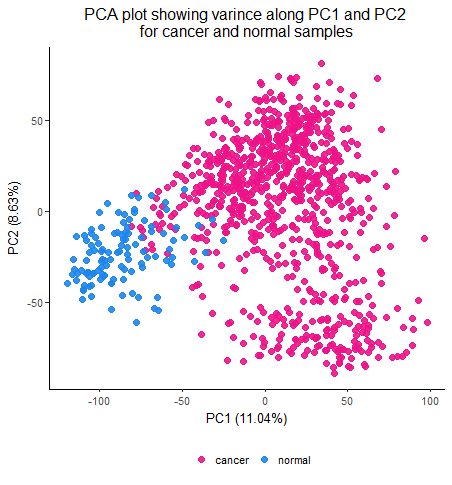
\includegraphics[scale=0.6]{pca_method.png}
            \caption{An example of PCA 2D scatter plot, showing the variance along PC1 and PC2 for cancer and normal samples}
            \label{fig:pcamethod}
            \end{figure}
        
    \newpage
    Another way of exploring variation characterised by PCA is to visualise variation of each principal component in a series of one-dimensional box plots. Figure \ref{fig:1dpcamethod} shows the variation seen in each PC (1-9) for the cancer/normal dataset shown as a scatter plot of first two PCs in Figure \ref{fig:pcamethod}. 
    In contrast, one-dimensional PCA plots are able to show variation along more than two PCs at a time. This method is useful for checking if any of the other PCs contain variation worth exploring. This is useful for checking for potential presence of batch effects or signatures left by other cofactors. 
    For each PC, the variation of each condition group, here - cancer and normal, is represented by a box plot. The PCs where condition boxes have the smallest overlap (e.g. PC1) will shows the clearest separation when plotted in 2D. 
       
    
        % PCA 1d
            \begin{figure}[h]
            \centering
            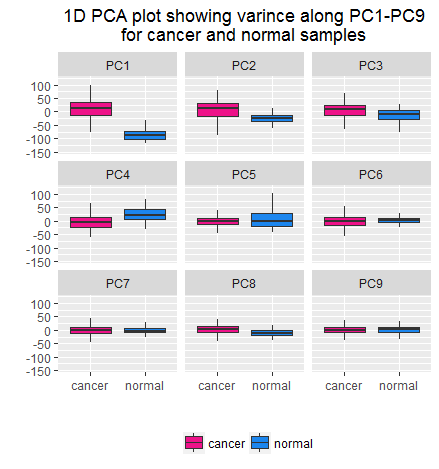
\includegraphics[scale=0.7]{1dpcamethod.png}
            \caption{An example of one-dimensional PCA plots for the cancer/normal dataset. }
            \label{fig:1dpcamethod}
            \end{figure}
   
  
    \subsection{Clustering and Heatmap representation}
    
    
    In clustering, or unsupervised classification, the aim is to identify subsets (clusters) in the data based on the similarity between single objects. Similar objects should be assigned to the same cluster, while objects which are not similar to each other, should be assigned to different clusters.
    Cluster analysis is applied to transcriptomics data to search for similar gene expression patterns between individual samples. This can help to reveal the data structure and give first insights into the data, which is especially useful if prior knowledge is little or non-existent. Clustering can, therefore, be seen as exploratory data analysis. 
        
    The purpose of clustering transcriptomics data is to statistically group samples according to their gene expression, in order to reduce complexity and dimensionality of the data, predict function or identify shared regulatory mechanisms \cite{Metsalu2015ClustVis:Heatmap}. Clustering can be performed as a part of heatmap. Heatmap is a datamatrix visualising values in the cells by the use of a color gradient. This gives a good overview of the largest and smallest values in the matrix. Rows (genes) and/or columns (samples) of the matrix are clustered to facilitate interpretation of sets of rows or columns rather than individual ones \cite{Metsalu2015ClustVis:Heatmap}.\\

    One of the popular methods is hierarchical clustering, which involves re-ordering of samples based on their distance in high dimensional space. The cluster is constructed based on the determination of two parameters — the distance metric and the linkage criterion.
    The two most common distance measures used for clustering are Euclidean and Manhattan distances. Typically the results of the two are quite similar, but most studies default to using the Euclidean measure. 
    The Euclidean distance involves computing the square root of square differences between two coordinates. In this way, the shortest path diagonally is calculated: $ \sqrt{(x_{1}-x_{2})^{2}+(y_{1}-y_{2})^{2}}$, where the first point is $(x1, y1)$ and the second point is $(x2, y2).$
    The Manhattan distance between two points is calculated by taking the sum of the lengths of the differences between the coordinates. Therefore, the distance is measure not in a straight line, but on horizontal (x) and vertical (y) axes — $ (x_{1}-x_{2})+(y_{1}-y_{2}).$
    
    Clustering works well when the data to be clustered is processed correctly. The low expressed genes have to be filtered out to remove non-informative noise after the counts data has been normalised and log2-transformed as will be discussed in section \ref{}, prior to clustering with the R function \texttt{hclust()} with default parameters. Hierarchical clustering on all genes was performed on all genes on data subgroup averages (Results section \ref{}).
    
    Heatmap clustering was performed on gene subsets, such as autophagy groups or $n$ genes with the highest variance (Results section \ref{}). The heatmaps were generated using Euclidean distance with avegare linkage (default) using the R package  \texttt{pheatmap} \cite{kolde2012pheatmap}.\\
    
    The results obtained for summarising the structure of transcriptomics data between PCA and clustering often show similar findings. For instance, if PCA shows a clear segregation of the data, clustering normally will support this.
    
    Figure \ref{fig:heatmapmethod} shows an example of unsupervised clustering of samples with heatmap. The data is clustered by columns (samples) and rows (genes), with dendograms showing how clusters are formed. The colour bar above the heatmap shows cancer/normal samples as pink/blue lines, and clustering forms blocks of colour. The heatmap colours  represent gene expression intensity according to the scale (high expression - dark blue, low expression - light yellow). This example shows how cancer and normal samples form two major clusters in the dendogram, which is noticeable in the heatmap colouring as well. Some of the samples are not within the expected clusters, i.e. are outliers, but that is OK, as some of mix up is seen in PCA too. 
    
            % PCA 1d
            \begin{figure}[h]
            \centering
            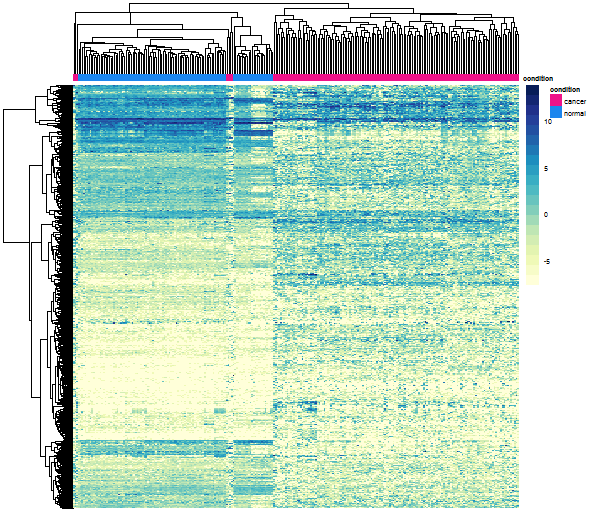
\includegraphics[scale=0.4]{heatmapmethod2.png}
            \caption{An example of clustering of the cancer/normal samples with heatmap representation. The data was clustered with Euclidean distance and average linkage. }
            \label{fig:heatmapmethod}
            \end{figure}
    
    
%     HCL implementing the Euclidean distance metric and the average linkage
% distance method to analyse the same data used to generate the PCA in figure 6
% determines that the data clusters into two predominant groups — one comprising
% all cancer samples and the other consisting of all control (healthy) samples. This
% indicates that the cancer transcriptomic profiles are more similar to each other
% than any of the control samples. These findings are reflected by those obtained
% from the PCA.
    
\newpage



\section{Hypothesis-driven analysis methods}    

    %why

    \subsection{Differential Expression Testing}
    
    %why
        \subsubsection{data preprocessing}
        \subsubsection{DE background}
        \subsubsection{limma}
        \subsubsection{multiple tesing correction}

    \subsection{Soft clustering}
        \subsubsection{prepossessing}
    
    \subsection{Enrichment Analysis}
    
    \subsection{PPi, TF, miRNA networks}